\section{Rational Expressions}
A quotient of two algebraic expressions is called a \textbf{fractional expression}. Here are
some examples:
$$ \frac{2x}{x-1} \quad \frac{y-2}{y^2+4} \quad \frac{x^3-x}{x^2+5x+6} \quad \frac{x}{\sqrt{x^2+1}}$$

A \textbf{rational expression} is a fractional expression in which both the numerator and the
denominator are polynomials. For example, the first three expressions in the above
list are rational expressions, but the fourth is not, since its denominator contains a
radical. In this section we learn how to perform algebraic operations on rational expressions.

\subsection{The Domain fo an Algebraic Expression}
In general, an algebraic expression may not be defined for all values of the variable.
The \textbf{domain} of an algebraic expression is the set of real numbers that the variable is
permitted to have. The table in the margin gives some basic expressions and their
domains

\begin{align*}
    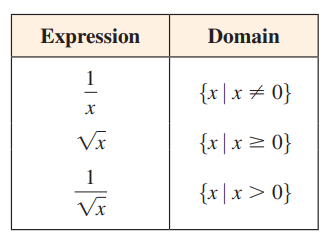
\includegraphics{algebra-pre-calculus/algebra/rational-expressions/expressions_domain.png}
\end{align*}

\subsection{Finding the Domain of an Expression}
Find the domains of the following expressions:
\textbf{(a)} $2x^2+3x-1$
This polynomial is defined for every x. Thus the domain is the set $\mathbb{R}$ of real
numbers. \\
\textbf{(b)} $\displaystyle \frac{x}{x^2-5x+6}$ \quad $\rightarrow$ We first factor the denominator. 
$$ x^2-5x+6 = (x-2)(x-3)$$ Since the denominator is zero when $x=2$ or $x=3$, the domain is the set of all real numbers except 2 and 3. So: $$ \text{Domain} = \{ x \in \mathbb{R} \mid x \neq 2, 3 \}$$
\\ \break 
\textbf{(c)} $\displaystyle \frac{\sqrt{x}}{x-5}$ \quad $\rightarrow$ For the numerator to b e defined, we must have $x\geq0$. Also we cannot we divide by zero, so $x\neq5$
Thus the domain is the set of all real numbers greater than or equal to zero, except 5. So: $$ \text{Domain} = \{ x \in \mathbb{R} \mid x \geq 0, x \neq 5 \}$$

\subsection{Simplifying Rational Expressions}
To \textbf{simplify rational expressions}, we factor both the numerator and the denominator and then \textbf{cancel} common factors from the numerator and denominator.
Like: $$ \frac{x^2-1}{x^2+x-2} = \frac{\cancel{(x-1)}(x+1)}{\cancel{(x-1)}(x-2)}=\frac{x+1}{x-2}$$


\subsection{Multiplying and Dividing Rational Expressions}
To \textbf{multiply rational expressions}, we are multiplying the numerators and denominators together. Like: $$ \frac{2x}{x^2-1} \cdot \frac{x^2-1}{x^2+1} = \frac{2x(x^2-1)}{(x^2-1)(x^2+1)} = \frac{2x}{x^2+1}$$ 

When it comes to \textbf{divide rational expressions}, we are multiplying the numerator by the reciprocal of the denominator. Like: $$ \frac{2x}{x^2-1} \div \frac{x^2-1}{x^2+1} = \frac{2x}{x^2-1} \cdot \frac{x^2+1}{x^2-1} = \frac{2x(x^2+1)}{(x^2-1)(x^2+1)} = \frac{2x}{x^2-1}$$

\subsection{Adding and Subtracting Rational Expressions}
To \textbf{add or subtract rational expressions}, we need to find a common denominator. We can do this by finding the least common multiple of the denominators. Like: $$ \frac{2}{x-1} + \frac{3}{x+1} = \frac{2(x+1)}{(x-1)(x+1)} + \frac{3(x-1)}{(x-1)(x+1)} = \frac{2x+2}{(x-1)(x+1)} + \frac{3x-3}{(x-1)(x+1)} = \frac{5x-1}{(x-1)(x+1)}$$

\subsection{Rationalizing the denominator or the Numerator}
If a fraction has a denominator of the form $A+B\sqrt{C}$, we can rationalize the denominator by multiplying numerator and denominator by the conjugate radical(its opposite) $A-B\sqrt{C}$.
This works because, by Special Product Formula 1, the product of the
denominator and its conjugate radical does not contain a radical:

$$ (A+B\sqrt{C})(A-B\sqrt{C})=A^2-B^2C$$

\subsection{Rationalizing the Denominator}
Rationalise the denominator: $\displaystyle \frac{1}{1+\sqrt{2}}$ \\ \break
We can multiply the numerator and denominator by the conjugate radical $1-\sqrt{2}$:
$$ \frac{1}{1+\sqrt{2}} \cdot \frac{1-\sqrt{2}}{1-\sqrt{2}} = \frac{1-\sqrt{2}}{1^2-(\sqrt{2})^2} = \frac{1-\sqrt{2}}{1-2} = \frac{1-\sqrt{2}}{-1} = \sqrt{2}-1$$
Here what we did is that we multiplied the numerator and denominator by the conjugate radical $1-\sqrt{2}$, then we simplified the denominator by using the Special Product Formula 1, and then we simplified the fraction.


\subsection{Rationalizing the Numerator}

Rationalise the numerator: $\displaystyle \frac{\sqrt{4+h}-2}{h}$ \\ \break
We can multiply the numerator and denominator by the conjugate radical $\sqrt{4+h}+2$:
$$ \frac{\sqrt{4+h}-2}{h} \cdot \frac{\sqrt{4+h}+2}{\sqrt{4+h}+2} = \frac{(\sqrt{4+h})^2-2^2}{h(\sqrt{4+h}+2)} = \frac{4+h-4}{h(\sqrt{4+h}+2)} = \frac{h}{h(\sqrt{4+h}+2)} = \frac{1}{\sqrt{4+h}+2}$$
Here what we did is that we multiplied the numerator and denominator by the conjugate radical $\sqrt{4+h}+2$, then we simplified the numerator by using the Special Product Formula 1, and then we simplified the fraction.


\subsection{Avoid Common Errors}
Don’t make the mistake of applying properties of multiplication to the operation of addition.
Many of the common errors in algebra involve doing just that. The following table states
several properties of multiplication and illustrates the error in applying them to addition.

\begin{align*}
    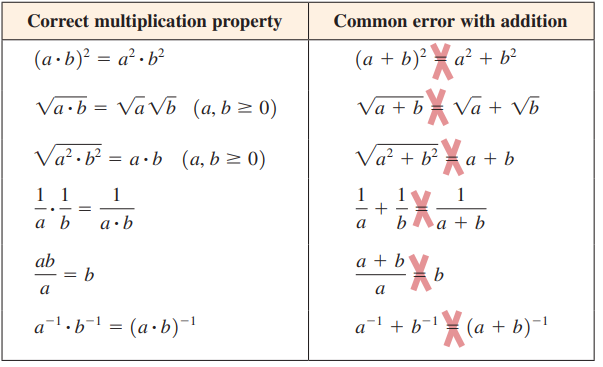
\includegraphics{algebra-pre-calculus/algebra/rational-expressions/common_errors.png}
\end{align*}

To verify that the equations in the right-hand column are wrong, simply substitute
numbers for a and b and calculate each side.